\documentclass{standalone}
\usepackage{pgfplots}
\usetikzlibrary{arrows.meta, decorations.markings}

% Set compatibility level for pgfplots
\pgfplotsset{compat=1.17}

\begin{document}

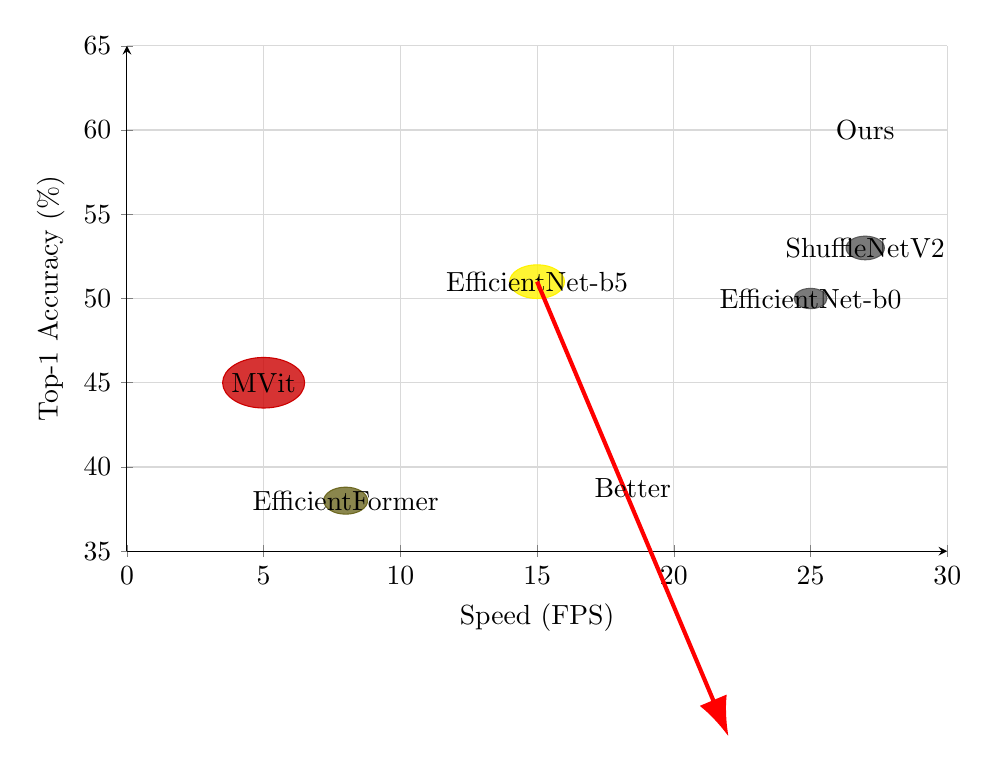
\begin{tikzpicture}
    \begin{axis}[
        xlabel={Speed (FPS)},
        ylabel={Top-1 Accuracy (\%)},
        xmin=0, xmax=30,
        ymin=35, ymax=65,
        xtick={0,5,...,30},
        ytick={35,40,...,65},
        grid=both,
        grid style={gray!30},
        axis lines=left,
        width=12cm,
        height=8cm,
        clip=false % To allow annotations outside the plot area
    ]

    % Draw the large red circle for MVit
    \filldraw[red!80!black, fill opacity=0.8] (5, 45) circle (1.5);

    % Draw the medium yellow circle for EfficientNet-b5
    \filldraw[yellow, fill opacity=0.8] (15, 51) circle (1.0);

    % Draw the small gray circle for ShuffleNetV2
    \filldraw[gray!70!black, fill opacity=0.8] (27, 53) circle (0.7);

    % Draw the small gray circle for EfficientNet-b0
    \filldraw[gray!70!black, fill opacity=0.8] (25, 50) circle (0.6);

    % Draw the small gray circle for EfficientFormer
    \filldraw[olive!70!black, fill opacity=0.8] (8, 38) circle (0.8);

    % Add node labels for each model
    \node[align=center] at (5, 45) {MVit};
    \node[align=center] at (15, 51) {EfficientNet-b5};
    \node[align=center] at (27, 53) {ShuffleNetV2};
    \node[align=center] at (25, 50) {EfficientNet-b0};
    \node[align=center] at (8, 38) {EfficientFormer};
    \node[align=center] at (27, 60) {Ours};

    % Draw the red arrow pointing towards better performance
    \draw[-{Latex[length=5mm]}, red, line width=1.5pt] 
        (15, 51) -- ++(7, 8) node[midway, above, black] {Better};

    % Add grid lines
    \end{axis}
\end{tikzpicture}

\end{document}